\documentclass[hyperref={pdfpagelabels=false},usepdftitle=false]{beamer}
\usepackage{../templates/myStyle}

\begin{document}
\selectlanguage{english}

\title{\titleText}
\subtitle{History of searching and the PageRank algorithm}
\author{\tutor}
\date{7th of February, 2013}
%\subject{Programmieren}

\frame{\titlepage}

\frame{
    \frametitle{Contents}
    \setcounter{tocdepth}{1}
    \tableofcontents
    \setcounter{tocdepth}{2}
}

%\AtBeginSection[]{
%    \InsertToC[sections={\thesection}]  % shows only subsubsections of one subsection
%}

\section{Introduction}
%!TEX root = Sommerakademie-2015-Forschung.tex
\section{Einleitung}
\subsection{Was ist On-Line Recognition?}

\begin{frame}{Demo}
    \begin{figure}[h]
        \centering
        \includegraphics*[width=0.7\linewidth, keepaspectratio]{images/Classification.png}
    \end{figure}

    \href{http://write-math.com}{write-math.com}
\end{frame}

\begin{frame}{Was ist On-Line Recognition?}
\medskip
\begin{columns}[t,onlytextwidth]
\begin{column}{.5\textwidth}
{\Large Off-line Recognition}
\begin{figure}[h]
    \centering
    \includegraphics*[width=0.7\linewidth, keepaspectratio]{images/A-pixel.png}
\end{figure}
\end{column}
\begin{column}{.5\textwidth}
{\Large On-line Recognition}
\begin{figure}[h]
    \centering
    \includegraphics*[width=0.7\linewidth, keepaspectratio]{images/A-vektor.png}
\end{figure}
\end{column}
\end{columns}
\end{frame}

\begin{frame}{Was wollen wir?}
    \[f(\text{Merkmale}) = \begin{pmatrix}0.7\\ 0.1\\ 0.2\end{pmatrix} = \begin{pmatrix} \mathbb{P}(\gamma)\\ \mathbb{P}(\text{ö})\\ \mathbb{P}(\heartsuit) \end{pmatrix}\]
    \medskip
    \visible<2->{
        \begin{center}
        {\Large Gesucht: Funktion $f$}\\
        (und Merkmalsextraktion)
    }
    \end{center}
\end{frame}

\begin{frame}{Merkmalsextraktion}
    \begin{figure}[h]
        \centering
        \includegraphics*[width=0.7\linewidth, keepaspectratio]{images/A-vektor-merkmalsbildung.png}
    \end{figure}

    Merkmalsvektor fester Länge ist praktisch
\end{frame}

\section{Funktionen}
\subsection{Funktionen}

\begin{frame}{Funktionen}
\begin{figure}[h]
    \centering
    \includegraphics*[width=0.7\linewidth, keepaspectratio]{images/function-machine.png}
\end{figure}
\end{frame}
\begin{frame}{Funktionen}
    \medskip
    \begin{columns}[t,onlytextwidth]
    \begin{column}{.5\textwidth}{
        \begin{itemize}[<+->]
            \item $f(x) = x^2$ ist $f: \mathbb{R} \rightarrow \mathbb{R}$
            \item $f(x, y) = x^2 + y^2$ ist $f: \mathbb{R}^2 \rightarrow \mathbb{R}$
            \item $f(x, y) = (x^2 + y^2, x \cdot y)$ ist $f: \mathbb{R}^2 \rightarrow \mathbb{R}^2$
        \end{itemize}
    }
    \end{column}
    \begin{column}{.4\textwidth}
    \only<1>{
        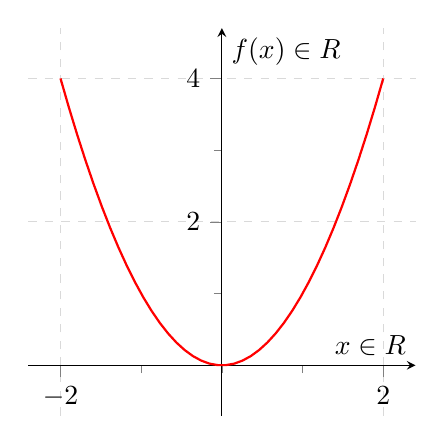
\begin{tikzpicture}
            \begin{axis}[
                legend pos=south west,
                axis x line=middle,
                axis y line=middle,
                grid = major,
                width=6.5cm,
                height=6.5cm,
                grid style={dashed, gray!30},
                xmin=-2,     % start the diagram at this x-coordinate
                xmax= 2,     % end   the diagram at this x-coordinate
                ymin=-0.25,  % start the diagram at this y-coordinate
                ymax= 4.25,  % end   the diagram at this y-coordinate
                axis background/.style={fill=white},
                xlabel=$x \in \mathbb{R}$,
                ylabel=$f(x) \in \mathbb{R}$,
                %xticklabels={-2,-1.6,...,7},
                %yticklabels={-8,-7,...,8},
                tick align=outside,
                minor tick num=-3,
                enlargelimits=true,
                tension=0.08]
              \addplot[domain=-2:2, red, thick,samples=40] {x*x};
            \end{axis}
        \end{tikzpicture}
    }
    \only<2->{
        \pgfplotsset{
            colormap={whitered}{
                color(0cm)=(white);
                color(1cm)=(orange!75!red)
            }
        }
        \begin{tikzpicture}
            \begin{axis}[
            colormap name=whitered,
            width=5.5cm,
            height=5.5cm,
            view={340}{25},
            enlargelimits=false,
            grid=major,
            domain=-3:3,
            y domain=-3:3,
            samples=56, %57 : TeX capacity exceeded, sorry [main memory size=3000000].
                        % see also http://tex.stackexchange.com/a/7954/5645
            xlabel=$x$,
            ylabel=$y$,
            zlabel={$f(x,y)$},
            ]
              \addplot3[surf] {x^2 + y^2};
            \end{axis}
        \end{tikzpicture}
    }
    \end{column}
    \end{columns}
\end{frame}

\begin{frame}{Funktionen mit Parametern}
    \begin{columns}
    \begin{column}{.5\textwidth}
        {\Large Mit Parametern}
        \begin{itemize}[<+->]
            \item $f(x) = x^2$
            \item $f(x) = 2 \cdot x^2$
            \item $f(x) = \nicefrac{1}{2} \cdot x^2$
            \item $f(x) = a \cdot x^2$
            \item $f(x_1, \dots, x_{166}) = \sum_{i=1}^{166} a_i \cdot x_i$\\
                  $\mathbb{R}^{166} \rightarrow \mathbb{R}$
            \item $f(x_1, \dots, x_{166}) = (\sum_{i=1}^{166} a_i \cdot x_i, \dots, \sum_{i=1}^{166} z_i \cdot x_i)$\\
                  $\mathbb{R}^{166} \rightarrow \mathbb{R}^{\text(\# Klassen)}$
        \end{itemize}
    \end{column}
    \begin{column}{.4\textwidth}
        \begin{tikzpicture}
            \begin{axis}[
                legend pos=south west,
                axis x line=middle,
                axis y line=middle,
                grid = major,
                width=6.5cm,
                height=6.5cm,
                grid style={dashed, gray!30},
                xmin=-2,     % start the diagram at this x-coordinate
                xmax= 2,     % end   the diagram at this x-coordinate
                ymin=-0.25,  % start the diagram at this y-coordinate
                ymax= 4.25,  % end   the diagram at this y-coordinate
                axis background/.style={fill=white},
                xlabel=$x \in \mathbb{R}$,
                ylabel=$f(x) \in \mathbb{R}$,
                %xticklabels={-2,-1.6,...,7},
                %yticklabels={-8,-7,...,8},
                tick align=outside,
                minor tick num=-3,
                enlargelimits=true,
                tension=0.08]
              \only<1->{\addplot[domain=-2:2, red, thick,samples=40] {x*x};}
              \only<2->{\addplot[domain=-2:2, blue, thick,samples=40] {2*x*x};}
              \only<3->{\addplot[domain=-2:2, green, thick,samples=40] {0.5*x*x};}
            \end{axis}
        \end{tikzpicture}
    \end{column}
    \end{columns}
\end{frame}

\begin{frame}{Fehlerfunktion}
    \begin{itemize}[<+->]
        \item \textbf{Daten $(x_{i,1}, \dots, x_{i,n}, y_{i,1}, \dots, y_{i,\text{\# Klassen}})$}: Beispiele für den Computer
        \item \textbf{Aktuelles Modell $f$}: Funktion mit vielen Parametern
        \item \textbf{Fehlerfunktion}: Wie gut ist $f$ für die vorhandenen
              Daten?
    \end{itemize}
\end{frame}

\begin{frame}{Fehlerfunktion}
    Abbildung von \textbf{Parameterraum} auf den Fehler ($\mathbb{R}_0^+$)
\end{frame}

\begin{frame}{Minimieren mit Ableitungen}
    \begin{figure}[h]
        \centering
        \includegraphics*[width=0.7\linewidth, keepaspectratio]{images/derivative-function.png}
    \end{figure}
\end{frame}

\begin{frame}{Gradientenabstieg}
    \begin{figure}[h]
        \centering
        \includegraphics*[width=0.7\linewidth, keepaspectratio]{images/gradient-descent.png}
    \end{figure}
\end{frame}


\section{Neuronale Netze}
\subsection{Neuronale Netze}
\begin{frame}{Neuronale Netze}{}
    \begin{itemize}[<+->]
        \item Menge von parametrisierten Funktionen
              $\mathbb{R}^n \rightarrow \mathbb{R}^{\text(\# Klassen)}$
        \item $\mathbb{R}^n$: Eingabe,\\z.B. Farbe von Pixel~1, Farbe von Pixel~2, \dots
        \item $\mathbb{R}^{\text(\# Klassen)}$: Ausgabe,\\Wahrscheinlichkeit der Klasse (z.B. 0, 1, 2, 3, 4, 5, 6, 7, 8, 9)
        \item Ableitbar
    \end{itemize}
\end{frame}

\section{Ausblick}
\subsection{Ausblick}
\begin{frame}{Ausblick}
    Erkennung von Formeln
    \begin{itemize}[<+->]
        \item Aufbau eines Sprachmodells der Mathematik
        \item Erweiterung der Symboldatenbank
        \item Segmentierung
    \end{itemize}
\end{frame}



\section{PageRank}
\subsection{How can we use this massive amout of information?}
\begin{frame}{How can we use this massive amout of information?}
    \begin{itemize}[<+->]
        \item 625.3 million websites
        \item Wikipedia is one website and has several millions of pages
        \item[$\Rightarrow$] we need to rank websites!
    \end{itemize}
\end{frame}

\subsection{Idea}
\begin{frame}{Basics of PageRank}
    We all know that:
    \begin{itemize}[<+->]
        \item humans know what is good for them
        \item[\xmark] machines don't know what's good for humans
        \item humans create websites
        \item humans will only \href{http://en.wikipedia.org/wiki/Hyperlink}{link} to websites they like
        \item[$\Rightarrow$] hyperlinks are a quality indicator
    \end{itemize}
\end{frame}

\begin{frame}{How Could We Use That?}
    \begin{itemize}[<+->]
        \item simply count number of links to a website
        \item[\xmark] 10,000 links from only one page
        \item count number of websites that link to a website
        \item[\xmark] quality of the linking website matters
        \item[\xmark] total number of links on the source page matters
    \end{itemize}
\end{frame}

\framedgraphic{A Brilliant Idea}{../images/BrinPage.jpg}

\begin{frame}{Ideas of PageRank}
    \begin{itemize}[<+->]
        \item decisions of humans are complicated
        \item a lot of webpages get visited
        \item[$\Rightarrow$] modellize clicks on links as random behaviour
        \item links are important
        \begin{itemize}
            \item links of page A get less important, if A has many links
            \item links of page A get more important, if many link to A
        \end{itemize}
        \item[$\Rightarrow$] if B has a link from A, the rank of B increases by $\frac{Rank(A)}{Links(A)}$
    \end{itemize}

    \pause[\thebeamerpauses]

    \begin{algorithmic}
        \If{A links to B}
            \State $Rank(B)$ += $\frac{Rank(A)}{Links(A)}$
        \EndIf
    \end{algorithmic}
\end{frame}

\begin{frame}{What is PageRank?}
    The PageRank algorithm calculates the probability of a randomly
    clicking user ending up on a given page.
\end{frame}

\begin{frame}
    \begin{figure}
        \begin{tikzpicture}[->,scale=1.8, auto,swap]
            % Draw the vertices. First you define a list.
            \foreach \pos/\name in {{(1,0)/a}, {(4,0)/b}, {(5,1)/c},
                                    {(3,1)/d}, {(4,2)/e}, {(5,2)/f},
                                    {(1,2)/g}, {(0,3)/h}, {(2,4)/i},
                                    {(4,3)/j}, {(4,4)/k}, {(5,4)/l}}
                \node[vertex] (\name) at \pos {$\name$};

            % Connect vertices with edges and draw weights
            \foreach \source/ \dest /\pos in {g/a/, b/c/bend right,
                c/b/bend right, d/e/bend right, e/d/, h/g/, g/i/,g/i/bend left, g/i/bend right,
                h/i/, h/i/bend left, g/j/bend right, j/g/,
                j/k/bend right, k/j/bend right, j/f/, f/l/,e/j/,
                l/l/loop right, j/d/}
                \path (\source) edge [\pos] node {} (\dest);
        \end{tikzpicture}
    \end{figure}
\end{frame}

\pgfdeclarelayer{background}
\pgfsetlayers{background,main}

\begin{frame}
    \begin{figure}
        \begin{tikzpicture}[->,scale=1.8, auto,swap]
            % Draw the vertices. First you define a list.
            \foreach \pos/\name in {{(1,0)/a}, {(4,0)/b}, {(5,1)/c},
                                    {(3,1)/d}, {(4,2)/e}, {(5,2)/f},
                                    {(1,2)/g}, {(0,3)/h}, {(2,4)/i},
                                    {(4,3)/j}, {(4,4)/k}, {(5,4)/l}}
                \node[vertex] (\name) at \pos {$15$};

            % Connect vertices with edges and draw weights
            \foreach \source/ \dest /\pos in {g/a/, b/c/bend right,
                c/b/bend right, d/e/bend right, e/d/, h/g/, g/i/,g/i/bend left, g/i/bend right,
                h/i/, h/i/bend left, g/j/bend right, j/g/,
                j/k/bend right, k/j/bend right, j/f/, f/l/,e/j/,
                l/l/loop right, j/d/}
                \path (\source) edge [\pos] node {} (\dest);

             \node<3->[vertex] (a) at (1,0) {$17$};
             \node<5->[vertex] (g) at (1,2) {$21$};
             \node<9->[vertex] (i) at (2,4) {$19$};

            \begin{pgfonlayer}{background}
                \path<2->[selected edge] (g.center) edge [] node {2} (a.center);
                \path<4->[selected edge] (j.center) edge [] node {6} (g.center);
                \path<6->[selected edge] (g.center) edge [bend left] node {1} (i.center);
                \path<7->[selected edge] (g.center) edge [] node {0} (i.center);
                \path<8->[selected edge] (g.center) edge [bend right] node {3} (i.center);
            \end{pgfonlayer}


        \end{tikzpicture}
    \end{figure}
\end{frame}


%\begin{frame}{Ants}
%    \begin{itemize}[<+->]
%        \item Websites = nodes = anthill
%        \item Links = edges = paths
%        \item You place ants on each node
%        \item They walk over the paths
%        \item[] (at random, they are ants!)
%        \item After some time, some anthills will have more ants than
%              others
%        \item Those hills are more attractive than others
%        \item \# ants is probability that a random user would end on
%              a website
%    \end{itemize}
%\end{frame}

\begin{frame}{Mathematics}
    Let $x$ be a web page. Then
    \begin{itemize}
        \item $L(x)$ is the set of websites that link to $x$
        \item $C(y)$ is the out-degree of page $y$
        \item $\alpha$ is probability of random jump
        \item $N$ is the total number of websites
    \end{itemize}

    \[\displaystyle PR(x) := \alpha \left ( \frac{1}{N} \right ) + (1-\alpha) \sum_{y\in L(x)} \frac{PR(y)}{C(y)}\]
\end{frame}

\begin{frame}{Pseudocode}
        \begin{algorithmic}
\alertline<1>             \Function{PageRank}{Graph $web$, double $q=0.15$, int $iterations$} %q is a damping factor
%\alertline<2>                 \ForAll{$page \in web$}
%\alertline<3>                     \State $page.pageRank = \frac{1}{|web|}$ \Comment{intial probability}
%\alertline<2>                 \EndFor

\alertline<2>                 \While{$iterations > 0$}
\alertline<3>                     \ForAll{$page \in web$} \Comment{calculate pageRank of $page$}
\alertline<4>                         \State $page.pageRank = q$
\alertline<5>                         \ForAll{$y \in L(page)$}
\alertline<6>                             \State $page.pageRank$ += $\frac{y.pageRank}{C(y)}$
\alertline<5>                         \EndFor
\alertline<3>                     \EndFor
\alertline<2>                     \State $iterations$ -= $1$
\alertline<2>                 \EndWhile
\alertline<1>             \EndFunction
        \end{algorithmic}
\end{frame}


\section{End}
\subsection{HWRT and write-math.com}
\begin{frame}{HWRT and write-math.com}
    Two software projects were created:
    \begin{itemize}
    \item \href{http://write-math.com}{write-math.com}: A website where
          on-line handwritten data gets collected and classified
    \item \href{https://github.com/MartinThoma/hwrt}{hwrt}: The
          \textit{handwriting recognition toolkit} is a Python project for
          handwriting recognition
    \end{itemize}

    This presentation and the bachelor's thesis will be at
    \href{http://martin-thoma.com/write-math/}{martin-thoma.com/write-math}.
\end{frame}

\subsection{Sources}
\begin{frame}{Image Sources}
    \begin{itemize}
	\item \href{https://commons.wikimedia.org/wiki/File:Server-multiple.svg}{Server} by RRZEicons
    \item \href{https://commons.wikimedia.org/wiki/File:Computer-aj_aj_ashton_01.svg}{Desktop Computer} by Ed g2s,
          Ironbrother, Kierancassel and Msgj
    \item \href{https://commons.wikimedia.org/wiki/File:Server_by_mimooh.svg}{Server} by Mimooh
    \end{itemize}
\end{frame}


\subsection{What You've Learned}
\begin{frame}{What You've Learned}
    \begin{itemize}
        \item web directories
        \item web crawler
        \item graph (nodes, eges)
        \item random walk (ants)
        \item PageRank
        \item read pseudocode
	\item filter bubble
    \end{itemize}
\end{frame}

\subsection{Sources}
\begin{frame}{Image Sources}
    \begin{itemize}
	\item \href{https://commons.wikimedia.org/wiki/File:Server-multiple.svg}{Server} by RRZEicons
    \item \href{https://commons.wikimedia.org/wiki/File:Computer-aj_aj_ashton_01.svg}{Desktop Computer} by Ed g2s,
          Ironbrother, Kierancassel and Msgj
    \item \href{https://commons.wikimedia.org/wiki/File:Server_by_mimooh.svg}{Server} by Mimooh
    \end{itemize}

    The presentation can be found at \url{http://tinyurl.com/write-math-short-presentation}
\end{frame}


\framedgraphic{Thanks for Your Attention!}{../images/Teach-yourself-C++-in-21-days.png}

\end{document}
